\documentclass[a4paper,12pt]{article}
\usepackage[utf8]{inputenc}
\usepackage[T1]{fontenc}
\usepackage[french]{babel}
\usepackage{graphicx}
\usepackage{hyperref}
\usepackage{geometry}
\geometry{margin=2.5cm}
\usepackage{setspace}
\onehalfspacing
\usepackage{graphicx}
\usepackage{float}

\begin{document}

% Page de garde
\begin{titlepage}
    \centering
    {\Large \textbf{Université Paris Nanterre}}\\[0.5cm]
    {\large Licence MIASHS - Parcours MIAGE}\\[0.2cm]
    {\large Semestre 4}\\[2cm]

    {\huge \textbf{Rapport de Projet}}\\[0.5cm]
    {\LARGE \textbf{Application de Planification de Voyages}}\\[0.5cm]
    {\LARGE \textit{"TravelDream"}}\\[2cm]

    \textbf{Réalisé par :}\\
    Melissa AKLI \\
    Nikola [Nom de famille] \\[0.5cm]

    \textbf{Encadré par :}\\
    Thibault Anani \\[2cm]

    \vfill
    \textbf{Année universitaire 2024-2025}
\end{titlepage}

\newpage
\tableofcontents
\newpage

\section{Introduction}

\subsection{Contexte du projet}
Dans le cadre du projet S4 de la licence MIASHS parcours MIAGE à l'Université Paris Nanterre, nous avons développé une application web nommée \textit{"TravelDream"} permettant aux utilisateurs de planifier leurs voyages de manière complète et organisée. Ce projet a été réalisé en binôme par Melissa et Nikola, et avait pour objectif de mettre en pratique nos compétences en développement web, en conception de bases de données et en modélisation. 
La planification de voyages est souvent une tâche complexe qui implique la gestion de nombreux éléments : transport, hébergement, activités, budget, etc. Notre application vise à centraliser toutes ces informations en un seul endroit, offrant ainsi aux utilisateurs un outil pratique pour organiser leurs déplacements et profiter pleinement de leurs expériences de voyage.
\subsection{Objectifs et problématique}
L'objectif principal de ce projet était de créer une plateforme interactive permettant aux utilisateurs de :
\begin{itemize}
    \item Gérer les voyages (dates, destinations)
    \item Organiser transports, hébergements, activités
    \item Suivre les dépenses
    \item Consulter une carte interactive
    \item Obtenir des recommandations via un assistant virtuel
\end{itemize}


La problématique centrale que nous avons cherché à résoudre est la suivante : comment simplifier et centraliser le processus de planification de voyage pour les utilisateurs, en leur offrant une interface intuitive et des fonctionnalités complètes ? Pour répondre à cette problématique, nous avons développé une application qui
combine :
\begin{itemize}
 \item Une base de données relationnelle bien structurée 
 \item Une interface utilisateur intuitive et responsive 
\item Des fonctionnalités adaptées aux besoins des voyageurs 
\item Des outils de visualisation comme la carte interactive
\item Un assistant virtuel pour guider les utilisateurs
\end{itemize}

\subsection{Méthodologie de travail}

Pour mener à bien ce projet, nous avons adopté une approche méthodique en plusieurs phases :

\begin{itemize}
  \item \textbf{Phase d'analyse :} Définition des besoins fonctionnels et non fonctionnels, création de personas et de cas d'utilisation pour comprendre les attentes des utilisateurs.
  
  \item \textbf{Phase de conception :} Élaboration du modèle conceptuel de données, conception du schéma relationnel de la base de données, et définition de l'architecture technique du projet.
  
  \item \textbf{Phase de développement :} Implémentation des fonctionnalités par modules (authentification, gestion des voyages, activités, etc.), développement de l'interface utilisateur, et intégration des différentes composantes.
  
  \item \textbf{Phase de test :} Vérification du bon fonctionnement des fonctionnalités, tests d'intégration, et correction des bugs identifiés.
  
  \item \textbf{Phase de finalisation :} Documentation du projet, préparation du rapport, et présentation des résultats.
\end{itemize}

Tout au long du projet, nous avons maintenu une communication constante entre les membres de l'équipe pour assurer la cohérence du développement et résoudre rapidement les problèmes rencontrés.

Dans les sections suivantes, nous détaillerons les différentes composantes de notre application, en commençant par l'analyse des besoins, puis en abordant la conception de la base de données, l'architecture technique, les fonctionnalités implémentées, et l'interface utilisateur.


\section{Analyse des Besoins}

\subsection{Besoins fonctionnels}

Notre application de planification de voyages \textit{TravelDream} a été conçue pour répondre à un ensemble de besoins fonctionnels précis, identifiés à partir des attentes des utilisateurs potentiels. Ces besoins définissent les capacités et services que notre système doit offrir :

\begin{itemize}
  \item \textbf{Gestion des utilisateurs}
  \begin{itemize}
    \item Création d'un compte utilisateur avec nom, email et mot de passe
    \item Connexion sécurisée
    \item Réinitialisation du mot de passe
    \item Déconnexion et gestion de session
  \end{itemize}

  \item \textbf{Gestion des voyages}
  \begin{itemize}
    \item Création d’un nouveau voyage (destination, dates)
    \item Consultation de la liste des voyages
    \item Modification des informations d’un voyage
    \item Suppression d’un voyage
  \end{itemize}

  \item \textbf{Gestion des activités}
  \item \textbf{Gestion des transports}
  \item \textbf{Gestion des logements}
  \item \textbf{Fonctionnalités supplémentaires}
  \begin{itemize}
    \item Carte interactive des destinations
    \item Assistant virtuel pour recommandations
  \end{itemize}
\end{itemize}


\subsection{Besoins non fonctionnels}

Au-delà des fonctionnalités, notre application devait également répondre à des exigences non fonctionnelles, qui définissent la qualité et les performances du système :

\begin{itemize}
  \item \textbf{Sécurité}
  \begin{itemize}
    \item Protection des données personnelles des utilisateurs
    \item Hachage des mots de passe pour éviter leur stockage en clair
    \item Utilisation de requêtes préparées pour prévenir les injections SQL
    \item Validation des entrées utilisateur pour éviter les attaques XSS
  \end{itemize}

  \item \textbf{Utilisabilité}
  \begin{itemize}
    \item Interface intuitive et facile à prendre en main
    \item Design responsive adapté aux différents appareils (ordinateurs, tablettes, smartphones)
    \item Temps de chargement rapide des pages
    \item Feedback visuel pour les actions utilisateur
  \end{itemize}

  \item \textbf{Performance}
  \begin{itemize}
    \item Optimisation des requêtes à la base de données
    \item Chargement efficace des ressources (images, scripts)
    \item Capacité à gérer plusieurs utilisateurs simultanément
  \end{itemize}

  \item \textbf{Maintenabilité}
  \begin{itemize}
    \item Code modulaire et bien structuré
    \item Séparation des préoccupations (modèle, vue, contrôleur)
    \item Documentation du code et des fonctionnalités
    \item Facilité d'extension pour ajouter de nouvelles fonctionnalités
  \end{itemize}

  \item \textbf{Fiabilité}
  \begin{itemize}
    \item Gestion appropriée des erreurs
    \item Validation des données côté serveur
    \item Persistance des données en cas d'erreur
  \end{itemize}
\end{itemize}

\subsection{Contraintes techniques}

Le développement de notre application a été soumis à plusieurs contraintes techniques, qui ont guidé nos choix technologiques et notre approche tout au long du projet :

\begin{itemize}
  \item \textbf{Environnement de développement}
  \begin{itemize}
    \item Utilisation de PHP pour le développement backend
    \item Base de données MySQL pour le stockage des données
    \item HTML, CSS et JavaScript pour le développement frontend
    \item Utilisation de Bootstrap pour le design responsive
  \end{itemize}

  \item \textbf{Infrastructure}
  \begin{itemize}
    \item Hébergement sur un serveur local pour le développement
    \item Configuration WAMP/MAMP pour l'environnement de développement
  \end{itemize}

  \item \textbf{Compatibilité}
  \begin{itemize}
    \item Support des navigateurs modernes (Chrome, Firefox, Safari, Edge)
    \item Adaptation aux différentes tailles d'écran
  \end{itemize}

  \item \textbf{Intégration}
  \begin{itemize}
    \item Utilisation de l'API Leaflet.js pour la carte interactive
    \item Intégration de l'API Nominatim pour la recherche de lieux
  \end{itemize}
\end{itemize}

\section{Conception de la Base de Données}
\section{Architecture Technique}

\subsection{Technologies utilisées}
Notre application de planification de voyages "TravelDream" a été développée en utilisant un ensemble de technologies modernes et complémentaires, choisies pour leur fiabilité, leur performance et leur adéquation avec les besoins du projet.

\paragraph{Backend}
\begin{itemize}
    \item \textbf{PHP 7.4} : Langage de programmation côté serveur utilisé pour développer la logique métier de l'application, gérer les sessions utilisateurs et interagir avec la base de données.
    \item \textbf{MySQL 8.0} : Système de gestion de base de données relationnelle utilisé pour stocker et gérer toutes les données de l'application.
    \item \textbf{PDO} : Extension PHP utilisée pour accéder à la base de
données de manière sécurisée, permettant l'utilisation de requêtes préparées pour prévenir les injections SQL.
\end{itemize}

\paragraph{Frontend}
\begin{itemize}
    \item \textbf{HTML5} : Langage de balisage utilisé pour structurer le contenu des pages web.
    \item \textbf{CSS3} : Langage de style utilisé pour définir la présentation visuelle des pages web.
    \item \textbf{JavaScript} : Langage de programmation côté client utilisé pour ajouter des fonctionnalités interactives aux pages web.
    \item \textbf{Bootstrap 5.3} : Framework CSS utilisé pour créer un design responsive et moderne, facilitant l'adaptation de l'interface à différentes tailles d'écran.
    \item \textbf{Font Awesome 6.4} : Bibliothèque d'icônes vectorielles utilisée pour améliorerl'interface utilisateur avec des icônes expressives.
\end{itemize}

\paragraph{APIs et bibliothèques externes}
\begin{itemize}
    \item \textbf{Leaflet.js} : Bibliothèque JavaScript open-source utilisée pour implémenter la carte interactive.
    \item \textbf{Nominatim API} : Service de géocodage utilisé pour la recherche de lieux sur la carte.
    \item \textbf{OpenStreetMap} : Fournisseur de données cartographiques utilisé comme fond de carte dans notre application.
\end{itemize}

\subsection{Structure du code}

Notre application suit une architecture modulaire qui sépare les différentes préoccupations du système, facilitant ainsi la maintenance et l'évolution du code.

\paragraph{Organisation générale}
Le code est organisé selon une structure proche du modèle MVC (Modèle-Vue-Contrôleur), bien que non strictement implémentée :
\begin{itemize}
    \item \textbf{Modèle} : Les interactions avec la base de données sont gérées principalement dans le fichier config.php qui contient des fonctions pour établir la connexion et effectuer des opérations courantes.
    \item \textbf{Vue} : Les fichiers PHP contenant principalement du HTML constituent la couche de présentation, avec l'aide des fichiers CSS pour le style.
    \item \textbf{Contrôleur} : La logique de traitement est intégrée dans les fichiers PHP principaux,
qui gèrent les requêtes utilisateur, traitent les données et préparent les réponses
\end{itemize}

\paragraph{Gestion des sessions}

La gestion des sessions utilisateur est implémentée de manière centralisée. Le fichier \texttt{header.php} initialise la session avec \texttt{session\_start()} et vérifie si l'utilisateur est connecté via la fonction \texttt{isUserLoggedIn()} définie dans \texttt{config.php}.

\vspace{0.5em}


\paragraph{Système de templates}
L'application utilise un système simple de templates avec des fichiers d'inclusion :
\begin{itemize}
  \item \texttt{header.php} : Contient l'en-tête HTML commun à toutes les pages, incluant les balises meta, les liens vers les feuilles de style et la barre de navigation.
  \item \texttt{footer.php} : Contient le pied de page commun et les scripts JavaScript.
\end{itemize}

Ces fichiers sont inclus dans chaque page de l'application, assurant ainsi une cohérence visuelle et fonctionnelle.

\subsection{Organisation des fichiers}
L'organisation des fichiers de notre projet suit une structure logique qui facilite la navigation et la maintenance du code.
\paragraph{Fichiers PHP principaux}
\begin{itemize}
    \item \texttt{config.php} : Contient les paramètres de configuration, les fonctions de connexion
à la base de données et diverses fonctions utilitaires.
     \item\texttt{header.php} : Gère l'en-tête des pages et la barre de navigation.
     \item\texttt{footer.php} : Gère le pied de page et l'inclusion des scripts JavaScript.
    \item \texttt{inscription.php} : Gère l'inscription des nouveaux utilisateurs.
     \item\texttt{pageconnexion.php} : Gère la connexion des utilisateurs existants.
     \item\texttt{Réinitialisation.php} : Permet aux utilisateurs de réinitialiser leur mot de passe.
     \item\texttt{logout.php} : Gère la déconnexion des utilisateurs.
    \item \texttt{destination.php}: Affiche les destinations populaires et permet la recherche.
     \item\texttt{mesvoyages.php}:  Affiche et gère les voyages de l'utilisateur connecté.
     \item\texttt{map.php} : Implémente la carte interactive avec géolocalisation. 
    \item \texttt{chat.php} : Implémente l'assistant virtuel de voyage.
\end{itemize}

\paragraph{Fichiers CSS}

Les fichiers CSS sont organisés par fonctionnalité ou par page :
\begin{itemize}
  \item \texttt{global.css} : Contient les styles globaux appliqués à l'ensemble de l'application.
  \item \texttt{style.css} : Contient les styles pour les pages d'authentification.
  \item \texttt{accueil.css} : Styles spécifiques à la page d'accueil.
  \item \texttt{destinations.css} : Styles pour la page des destinations.
  \item \texttt{profil\_new.css} : Styles pour la page de profil utilisateur.
  \item \texttt{chatbot.css} : Styles pour l'interface de l'assistant virtuel.
  \item \texttt{map.css} : Styles pour la carte interactive.
\end{itemize}

\vspace{0.5em}
\subsection{Configuration du système}

\paragraph{Configuration de la base de données}
La configuration de la connexion à la base de données est centralisée dans le fichier \texttt{config.php} :
\begin{figure}[H]
    \centering
    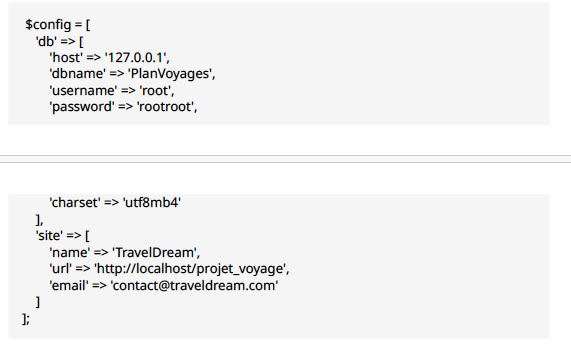
\includegraphics[width=0.8\textwidth]{capture1.png}
\end{figure}
Cette approche permet de modifier facilement les paramètres de connexion sans avoir à
modifier chaque fichier qui interagit avec la base de données.

\paragraph{Fonction de connexion à la base de données}
La fonction getDbConnection() dans config.php établit une connexion PDO à la base de données :
\begin{figure}[H]
  \centering
  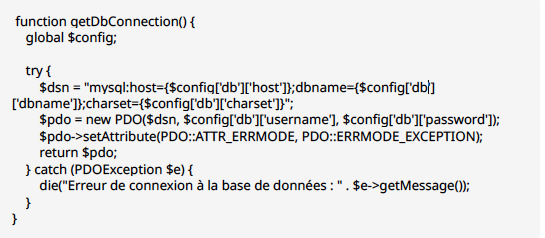
\includegraphics[width=0.95\textwidth]{capture2.png}
\end{figure}
Cette fonction configure également PDO pour qu'il lance des exceptions en cas d'erreur,facilitant ainsi le débogage.

\paragraph{Fonctions utilitaires}
Le fichier \texttt{config.php} contient également plusieurs fonctions utilitaires importantes
\begin{itemize}
    \item \texttt{isUserLoggedIn()} : Vérifie si l'utilisateur est connecté en contrôlant la présence de
l'ID utilisateur dans la session.
    \item \texttt{redirect()} : Facilite la redirection vers une autre page.
    \item \texttt{sanitize()} : Nettoie les données d'entrée pour prévenir les attaques XSS.
    \item \texttt{generateAlert()} : Génère des messages d'alerte formatés avec Bootstrap
    \item \texttt{formatDate()} : Formate les dates selon le format spécifié.
\end{itemize}

\subsection{Sécurité}
Plusieurs mesures de sécurité ont été mises en place :
\begin{itemize}
    \item Requêtes préparées (PDO) pour éviter les injections SQL.
    \item Mots de passe hachés avec \texttt{password\_hash()}.
    \item Nettoyage des entrées avec \texttt{sanitize()}.
    \item Gestion des sessions pour contrôler l'accès aux pages protégées.
\end{itemize}

Cette architecture technique robuste et bien organisée a permis de développer une
application fonctionnelle, sécurisée et facile à maintenir, tout en offrant une expérience
utilisateur fluide et agréable.

\section{Fonctionnalités Implémentées}

\subsection{Module d'Authentification}

Le module d'authentification constitue la porte d'entrée de notre application et assure la sécurité des données utilisateurs.  
Il comprend quatre fonctionnalités principales : l'inscription, la connexion, la réinitialisation du mot de passe et la déconnexion.

\subsubsection{Inscription}

La page d'inscription (\texttt{inscription.php}) permet aux nouveaux utilisateurs de créer un compte sur la plateforme.  
Cette fonctionnalité a été implémentée avec une attention particulière à la sécurité et à l'expérience utilisateur.

\paragraph{Processus d'inscription}

\begin{enumerate}
  \item L'utilisateur accède au formulaire d'inscription via le lien \og inscription  \fg{} dans la barre de navigation.
  \item Il remplit les champs requis : nom d'utilisateur, adresse email et mot de passe.
  \item À la soumission, le système vérifie si l'email est déjà utilisé.
  \item Si l'email est disponible, le mot de passe est haché via \texttt{password\_hash()} avant d’être stocké.
  \item Un message de confirmation s’affiche, invitant l’utilisateur à se connecter.
\end{enumerate}

\paragraph{Sécurité}

\begin{itemize}
  \item Utilisation de requêtes préparées pour prévenir les injections SQL.
  \item Hachage du mot de passe avec \texttt{bcrypt} via \texttt{password\_hash()}.
  \item Validation des données côté serveur.
\end{itemize}

\begin{figure}[H]
  \centering
  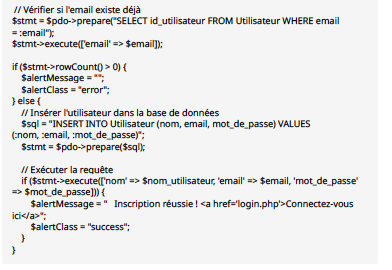
\includegraphics[width=0.9\textwidth]{capture3.png}
\end{figure}
\subsubsection{Connexion}

La page de connexion (\texttt{pageconnexion.php}) permet aux utilisateurs existants d'accéder à leur compte et à leurs données personnelles.

\paragraph{Processus de connexion}

\begin{enumerate}
  \item L'utilisateur accède au formulaire de connexion via le lien \og Connexion \fg{} dans la barre de navigation.
  \item Il saisit son adresse email et son mot de passe.
  \item Le système vérifie l'existence de l'email dans la base de données.
  \item Si l'email existe, le mot de passe est vérifié via \texttt{password\_verify()}.
  \item En cas de succès, les données de l’utilisateur sont stockées en session, puis il est redirigé vers son profil.
  \item En cas d’échec, un message d’erreur est affiché.
\end{enumerate}

\paragraph{Gestion de session}

Après une connexion réussie, les informations suivantes sont stockées en session :
\begin{itemize}
  \item ID de l'utilisateur
  \item Nom d'utilisateur
  \item Adresse email
\end{itemize}

Cela permet d’identifier l’utilisateur et de personnaliser son expérience.

\begin{figure}[H]
  \centering
  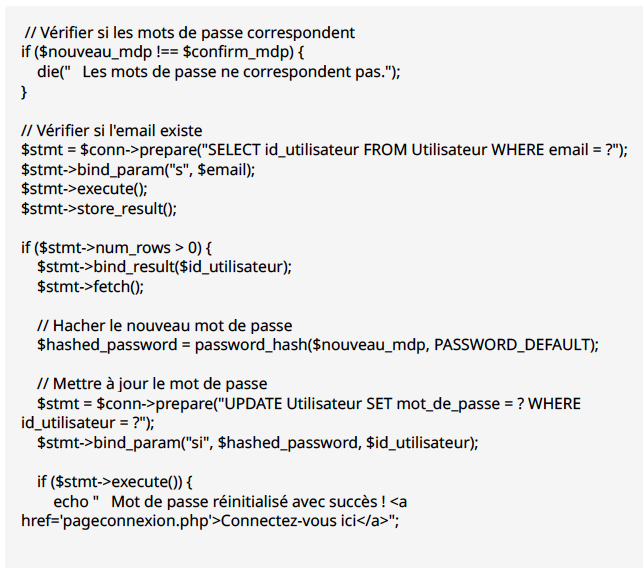
\includegraphics[width=0.9\textwidth]{capture4.png}
\end{figure}
\subsubsection{Réinitialisation du mot de passe}
La fonctionnalité de réinitialisation du mot de passe (\texttt{Reinitialisation.php}) permet aux utilisateurs ayant oublié leur mot de passe de le réinitialiser de manière sécurisée.

\textbf{Processus de réinitialisation}
\begin{itemize}
  \item L'utilisateur accède au formulaire de réinitialisation via le lien \og Mot de passe oublié \fg{} sur la page de connexion.
  \item Il saisit son adresse email, un nouveau mot de passe et la confirmation de ce mot de passe.
  \item Le système vérifie que les deux mots de passe correspondent.
  \item Si l'email existe dans la base de données, le nouveau mot de passe est haché et mis à jour.
  \item Un message de confirmation s'affiche et l'utilisateur est invité à se connecter avec son nouveau mot de passe.
\end{itemize}

\textbf{Sécurité}
\begin{itemize}
  \item Vérification de la correspondance des mots de passe saisis.
  \item Hachage du nouveau mot de passe avant stockage.
  \item Utilisation de requêtes préparées pour la mise à jour en base de données.
\end{itemize}

\subsubsection{Déconnexion}
La fonctionnalité de déconnexion ( logout.php ) permet aux utilisateurs de se
déconnecter en toute sécurité de leur compte. 
\paragraph{Processus de déconnexion}
\begin{enumerate}
  \item L'utilisateur clique sur le lien \og Déconnexion \fg{} dans la barre de navigation.
  \item Le script détruit la session en cours, effaçant toutes les variables de session.
  \item L'utilisateur est redirigé vers la page de connexion.
\end{enumerate}

\paragraph{Sécurité}
\begin{itemize}
  \item Destruction complète de la session pour éviter tout accès non autorisé.
  \item Redirection immédiate pour empêcher toute action après la déconnexion.
\end{itemize}
\begin{figure}[H]
  \centering
  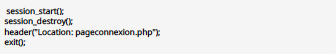
\includegraphics[width=0.9\textwidth]{capture5.png}
  \caption{Interface de la page de connexion}
\end{figure}
\section{Gestion des Voyages}
\subsection{ Visualisation des voyages}

La page \texttt{mesvoyages.php} permet aux utilisateurs de consulter l'ensemble de leurs voyages planifiés, en cours ou passés.

\textbf{Fonctionnalités} :
\begin{itemize}
  \item Affichage de la liste des voyages de l'utilisateur, triés par date de début (du plus récent au plus ancien).
  \item Pour chaque voyage : destination, dates de début et de fin, durée.
  \item Indication visuelle du statut du voyage : à venir, en cours, terminé.
  \item Statistiques : nombre total de voyages, destinations uniques, total de jours de voyage.
  \item Affichage du prochain voyage et du nombre de jours restants.
\end{itemize}
\subsection{Carte interactive}
\subsection*{5.6.1 Carte interactive}

La carte interactive (\texttt{map.php}) permet aux utilisateurs de visualiser et de rechercher des lieux sur une carte mondiale.

\textbf{Fonctionnalités} :
\begin{itemize}
  \item Affichage d'une carte interactive utilisant Leaflet.js et OpenStreetMap.
  \item Recherche de lieux via l'API Nominatim.
  \item Géolocalisation pour afficher la position actuelle de l'utilisateur.
  \item Ajout de marqueurs sur les lieux recherchés.
\end{itemize}

\textbf{Implémentation technique} :
\begin{itemize}
  \item \textbf{Initialisation de la carte} :
  \begin{figure}[H]
  \centering
  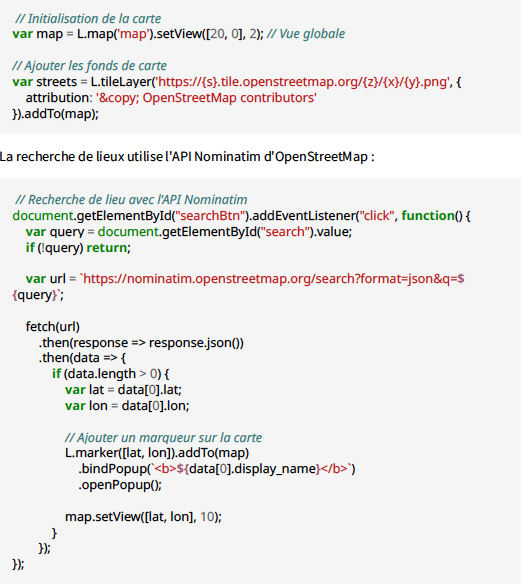
\includegraphics[width=0.9\textwidth]{1.png}
  
\end{figure}

  \item \textbf{Géolocalisation avec l'API navigateur} :
  \begin{figure}[H]
  \centering
  \includegraphics[width=0.9\textwidth]{Capture d’écran 2025-05-16 à 12.50.04.png}
 
\end{figure}
\end{itemize}

\subsection{Assistant de voyage (chatbot)}

L'assistant de voyage (\texttt{chat.php}) est un chatbot intelligent qui aide les utilisateurs à trouver des destinations adaptées à leurs préférences.

\paragraph{Fonctionnalités}
\begin{itemize}
  \item Interface de chat intuitive.
  \item Base de données de destinations avec leurs caractéristiques (climat, budget, activités, etc.).
  \item Algorithme de recommandation basé sur les préférences exprimées par l'utilisateur.
  \item Présentation des destinations recommandées avec leurs informations principales.
\end{itemize}

\paragraph{Implémentation technique}
L’assistant est implémenté en JavaScript côté client avec une base de données locale.

\begin{figure}[H]
  \centering
  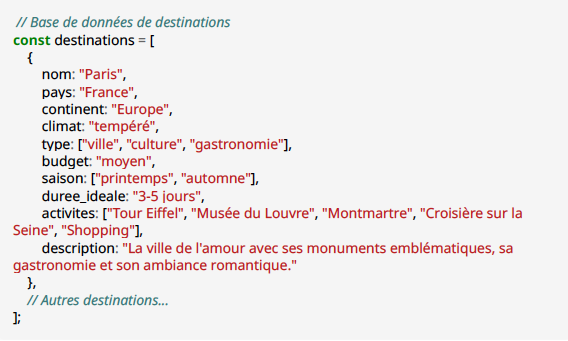
\includegraphics[width=0.9\textwidth]{capture6.png}
\end{figure}
L'algorithme de recommandation filtre les destinations selon les préférences de
l'utilisateur :
\begin{figure}[H]
  \centering
  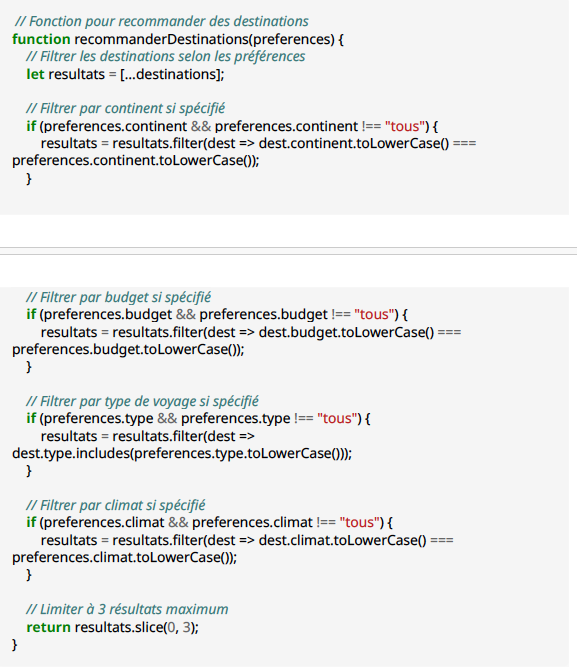
\includegraphics[width=0.9\textwidth]{capture7.png}
\end{figure}
\subsection{Recherche de destinations (destination.php)}

Cette fonctionnalité permet aux utilisateurs de découvrir des lieux de voyage populaires et d’obtenir des informations détaillées sur ceux-ci.

\paragraph{Fonctionnalités}
\begin{itemize}
  \item Affichage des destinations populaires avec images et descriptions.
  \item Barre de recherche pour trouver une destination spécifique.
  \item Affichage détaillé (meilleure période, budget, activités recommandées).
  \item Possibilité de planifier directement un voyage vers la destination choisie.
\end{itemize}

\paragraph{Implémentation technique}
Les informations sont définies dans le code PHP

\begin{figure}[H]
  \centering
  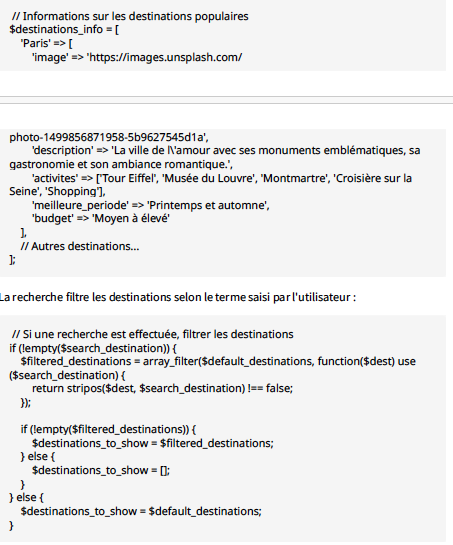
\includegraphics[width=0.9\textwidth]{capture8.png}
\end{figure}
\section{Interface Utilisateur}

\subsection{Charte graphique}
L’interface de l’application \textbf{TravelDream} a été conçue pour offrir une expérience utilisateur agréable, fluide et cohérente. Elle repose sur une charte graphique harmonieuse appliquée à l’ensemble du site.

\subsubsection{Palette de couleurs}
\begin{itemize}
  \item \textbf{Couleur principale} : Bleu ciel (\#4A89DC) – Évoque le ciel, l’océan et la liberté.
  \item \textbf{Couleur secondaire} : Vert tendre (\#48CFAD) – Symbolise la nature et les paysages.
  \item \textbf{Couleur d’accentuation} : Orange (\#FC6E51) – Représente le soleil et l’énergie.
  \item \textbf{Couleurs neutres} : 
  \begin{itemize}
    \item Blanc (\#FFFFFF) – Fond principal pour une lecture confortable.
    \item Gris clair (\#F5F7FA) – Fond secondaire pour distinguer certaines sections.
    \item Gris foncé (\#434A54) – Texte principal pour un bon contraste.
  \end{itemize}
\end{itemize}

\subsubsection{Typographie}
\begin{itemize}
  \item \textbf{Titres} : Montserrat – Moderne, sans-serif, excellente lisibilité.
  \item \textbf{Corps de texte} : Open Sans – Clair et fluide pour le contenu principal.
  \item \textbf{Accents décoratifs} : Pacifico – Cursive utilisée avec parcimonie.
\end{itemize}

\paragraph{Hiérarchie des tailles}
\begin{itemize}
  \item Titres principaux (h1) : 2.5rem
  \item Sous-titres (h2) : 2rem
  \item Titres de section (h3) : 1.5rem
  \item Corps de texte : 1rem
  \item Texte secondaire : 0.875rem
\end{itemize}

\subsubsection{Iconographie}
Nous utilisons la bibliothèque \textbf{Font Awesome} pour des icônes vectorielles adaptables à tous les supports.

\textbf{Utilisations principales :}
\begin{itemize}
  \item Illustration des fonctionnalités (ex : avion, lit)
  \item Navigation (flèches, menu hamburger)
  \item Actions (ajout, modification, suppression)
  \item Statuts (succès, erreur, information)
\end{itemize}

\subsubsection{Éléments d’interface}
\begin{itemize}
  \item \textbf{Boutons} : Coins arrondis, couleur d’action (primaire, secondaire, danger), icône si besoin.
  \item \textbf{Cartes} : Coins arrondis, ombre légère, marges internes.
  \item \textbf{Formulaires} : Champs avec bordures fines, labels clairs, retour visuel de validation.
  \item \textbf{Alertes} : Couleurs distinctes selon le type (succès, erreur, info, avertissement).
\end{itemize}
\subsection{Maquettes et wireframes}

Avant le développement, des maquettes et wireframes ont été réalisés afin de structurer l’interface et garantir une navigation fluide et cohérente.

\subsubsection{Page d'accueil et destinations}

La page d'accueil présente une image de fond évocatrice avec un message d'accueil et
une barre de recherche proéminente. En dessous, on trouve une sélection de
destinations populaires présentées sous forme de cartes avec images.
\begin{figure}[H]
    \centering
    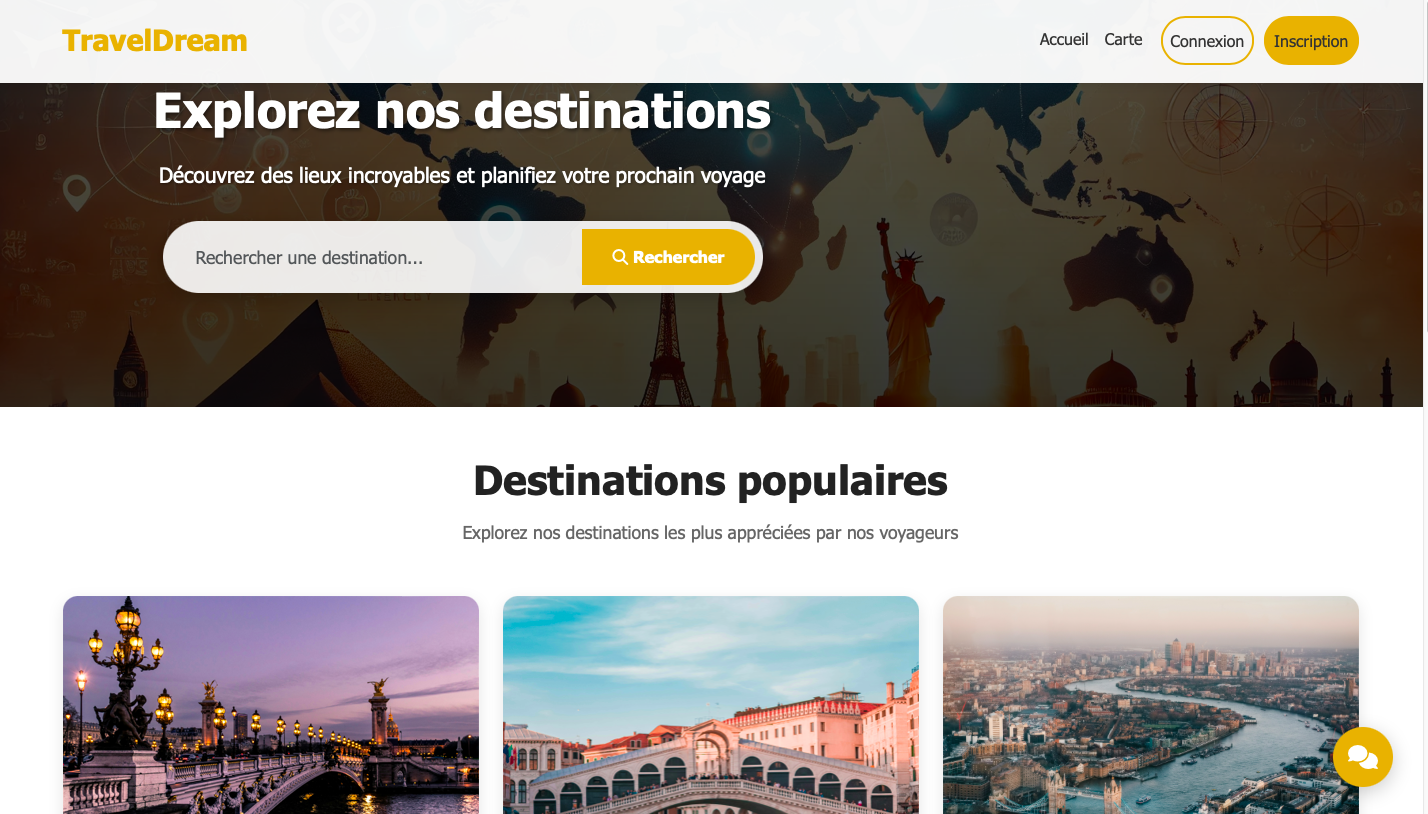
\includegraphics[width=0.8\textwidth]{Destination.png}
\end{figure}

\vspace{0.5cm}
\subsubsection{Pages d'authentification}
Les pages de connexion et d'inscription partagent une structure similaire avec un
formulaire simple sur un fond d'image de voyage. Cette approche minimaliste permet à
l'utilisateur de se concentrer sur l'action à effectuer.
\begin{figure}[H]
    \centering
    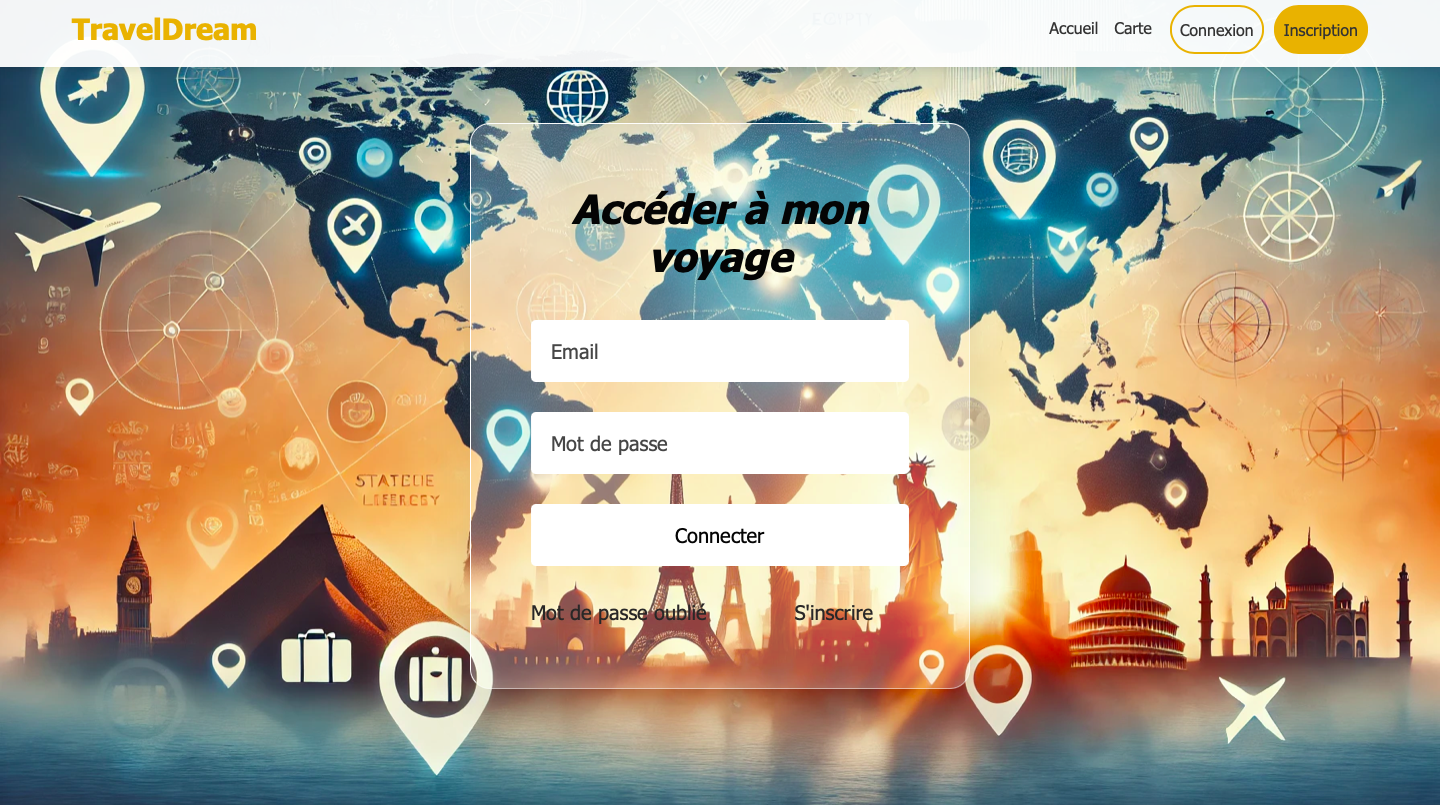
\includegraphics[width=0.8\textwidth]{accueil.png}
\end{figure}
\subsubsection{Profil et gestion des voyages}
La page de profil est divisée en deux sections principales : un résumé du profil avec
statistiques à gauche, et la liste des voyages à droite. Chaque voyage est présenté dans
une carte contenant les informations essentielles et des boutons d'action.
\begin{figure}[H]
    \centering
    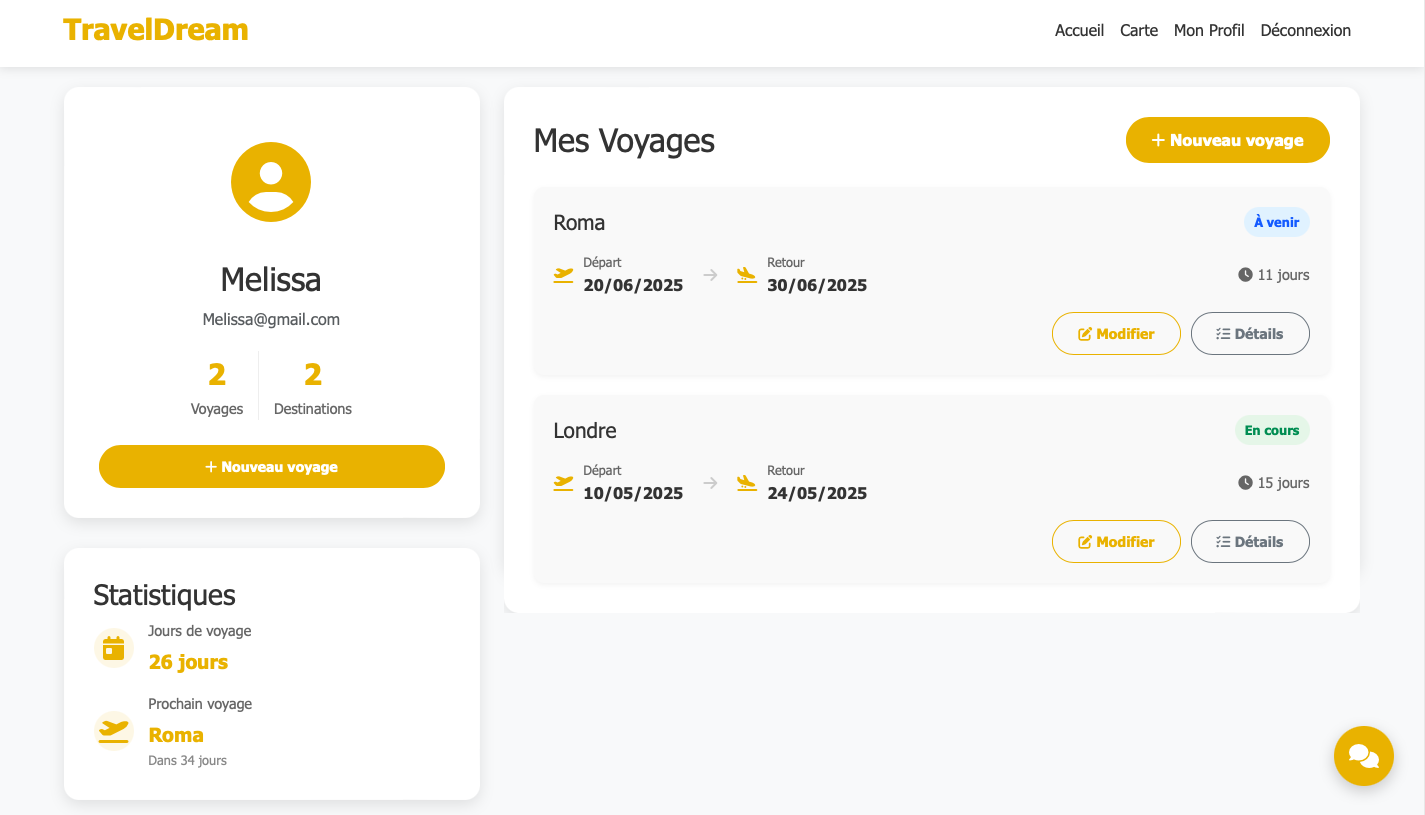
\includegraphics[width=0.8\textwidth]{profil.png}
\end{figure}
\subsubsection{Carte interactive}
La carte interactive occupe la majeure partie de l’écran et inclut :
\begin{itemize}
  \item Une barre de recherche en haut.
  \item Des boutons de contrôle pour zoom, filtres, etc.
\end{itemize}
\begin{figure}[H]
    \centering
    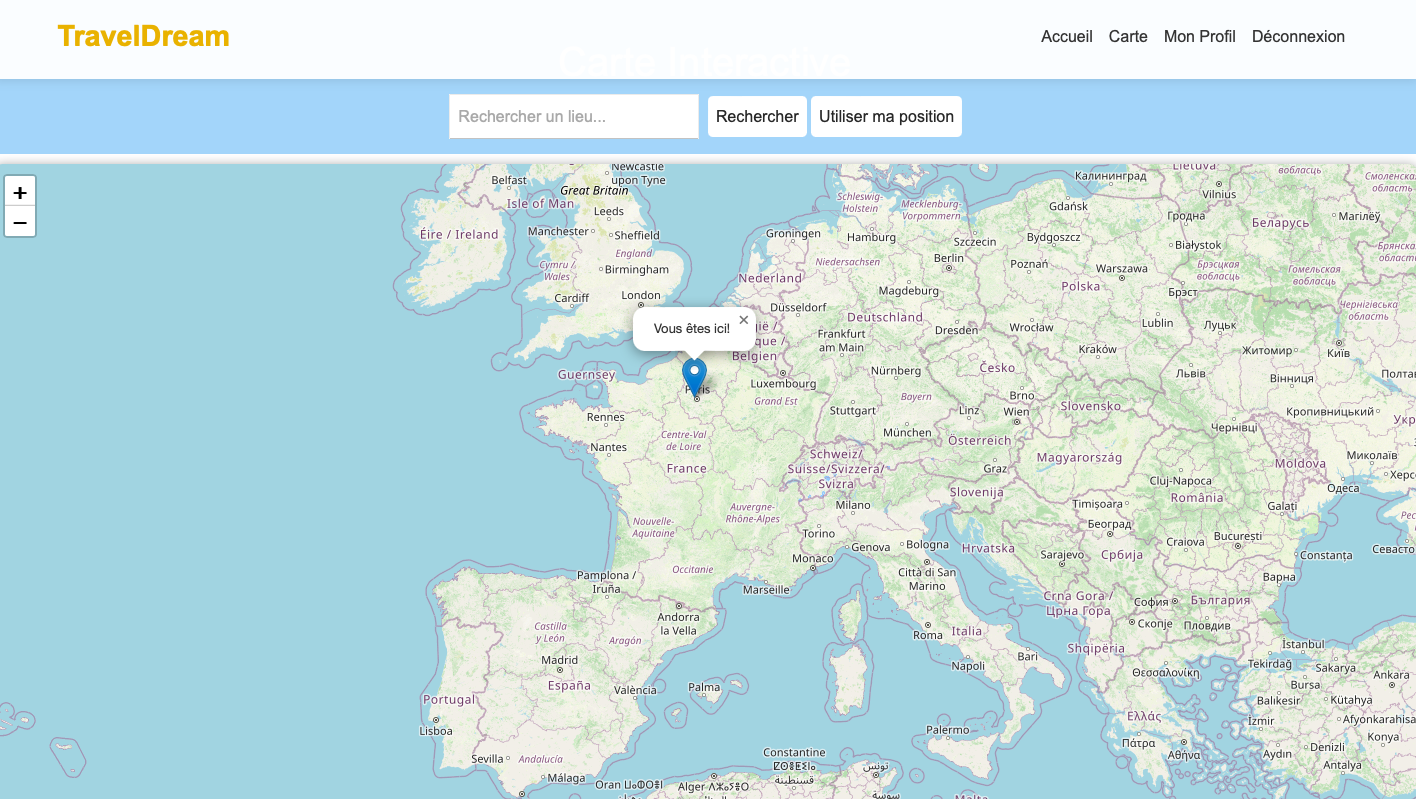
\includegraphics[width=0.8\textwidth]{carte.png}
\end{figure}
\subsubsection{Assistant de voyage (chatbot)}
L'interface de l'assistant de voyage (chatbot) présente une zone de chat à droite et une
zone d'information à gauche, créant un équilibre visuel tout en maintenant la
fonctionnalité.
\begin{figure}[H]
    \centering
    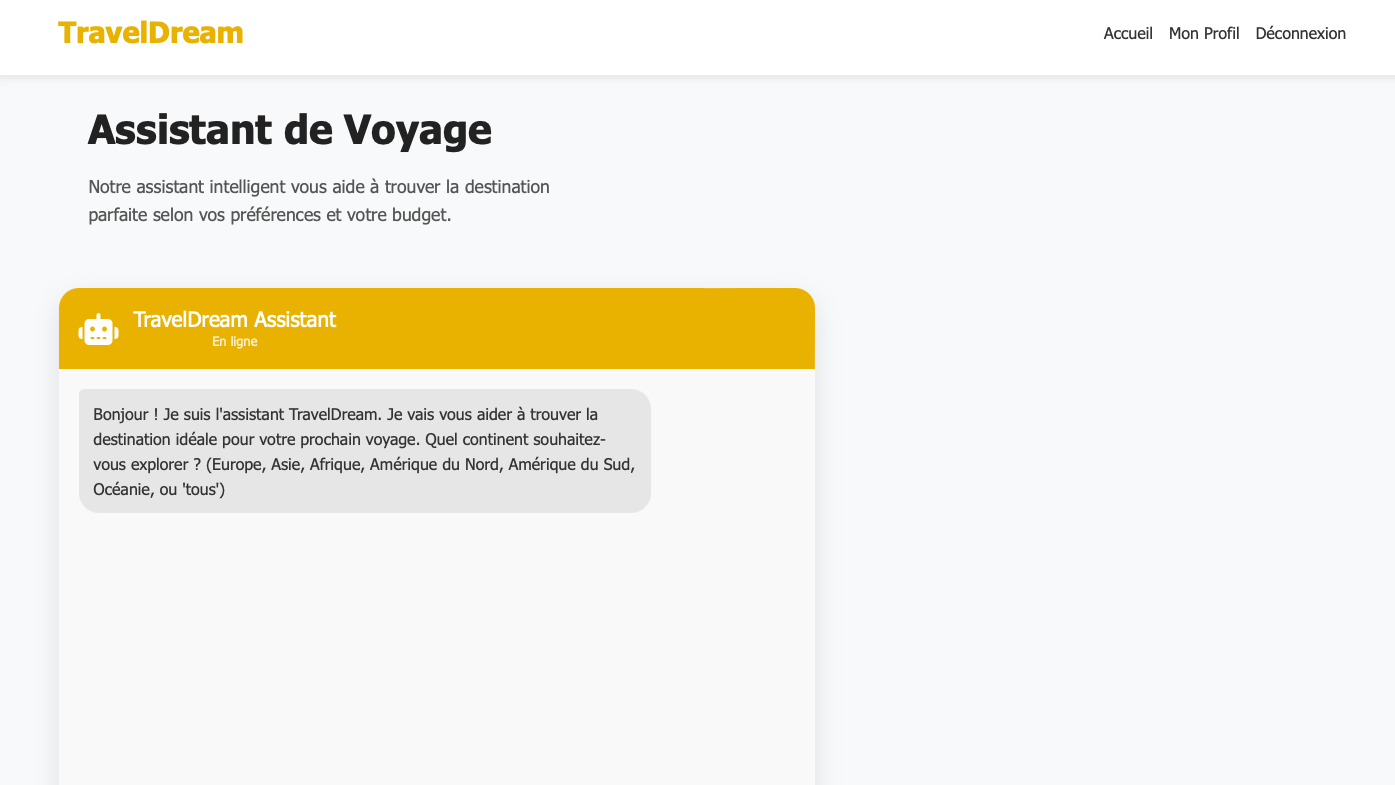
\includegraphics[width=0.8\textwidth]{chat.png}
\end{figure}
\subsection{Responsive Design}
Notre application a été conçue selon les principes du "mobile-first" et du design
responsive, garantissant une expérience utilisateur optimale sur tous les appareils, des
smartphones aux grands écrans d'ordinateur.
\begin{figure}[H]
    \centering
    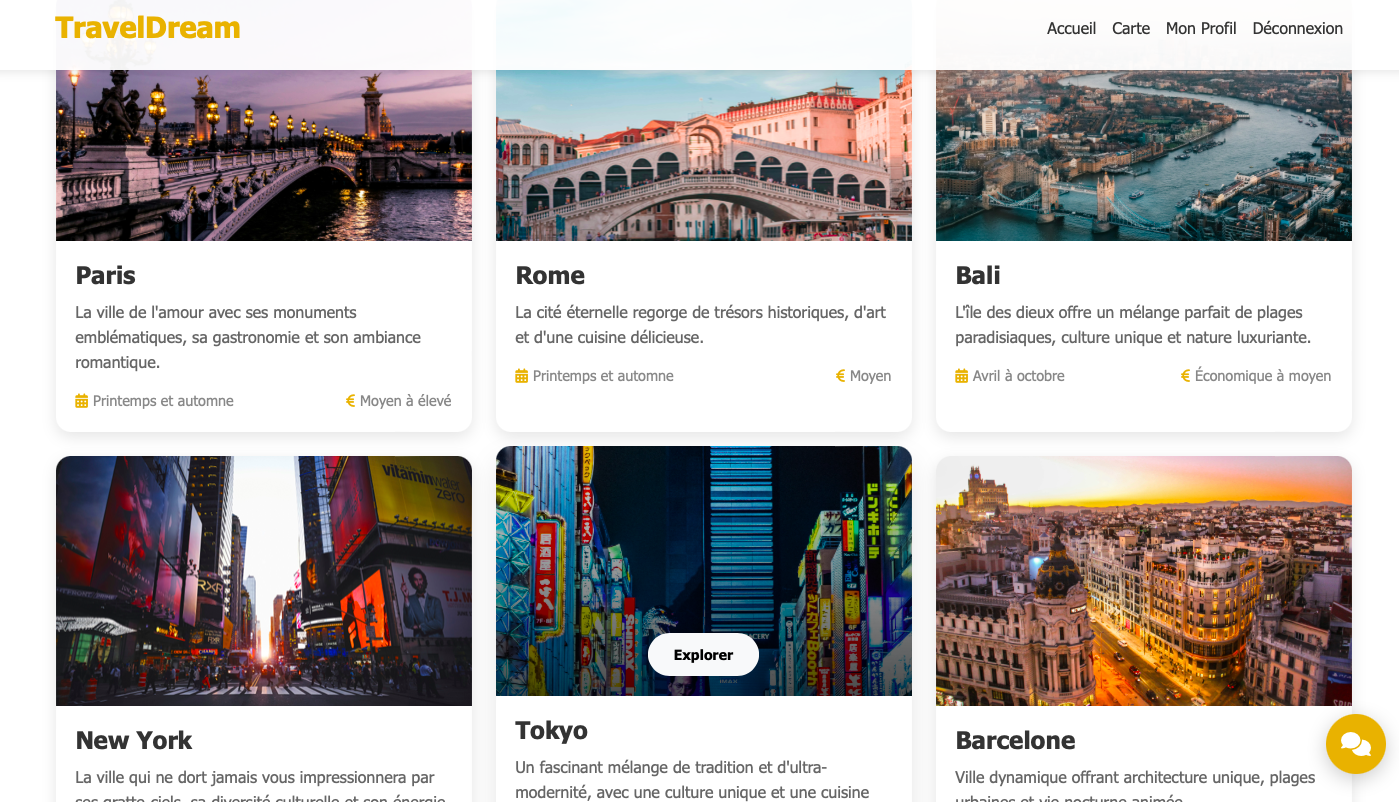
\includegraphics[width=0.8\textwidth]{design.png}
\end{figure}

\subsubsection{Approche technique}
Nous avons utilisé Bootstrap 5 pour garantir une mise en page adaptable :
\begin{itemize}
  \item Système de grille 12 colonnes.
  \item Media queries pour adapter l’affichage.
  \item Classe \texttt{img-fluid} pour rendre les images responsives.
  \item Composants modulables selon la taille d’écran.
\end{itemize}

\subsubsection{Adaptations spécifiques}
Des ajustements ont été appliqués pour améliorer l’expérience utilisateur :
\begin{itemize}
  \item Menu hamburger sur petits écrans.
  \item Cartes de voyage : 3 colonnes (desktop), 2 (tablette), 1 (mobile).
  \item Réorganisation verticale des sections sur mobile.
  \item Champs de formulaire adaptés en largeur.
\end{itemize}

\section{Tests et Validation}

\subsection{Stratégie de test}
Pour garantir la qualité et la fiabilité de notre application \textit{TravelDream}, nous avons mis en place une stratégie de test complète couvrant différents aspects du système. Cette approche méthodique nous a permis d'identifier et de corriger les problèmes avant le déploiement final.

\subsubsection{Types de tests implémentés}
Notre stratégie a intégré plusieurs types de tests :
\begin{itemize}
  \item \textbf{Tests unitaires} : vérification du bon fonctionnement de chaque composant (fonctions, classes, modules)
  \item \textbf{Tests d'intégration} : validation des interactions entre les différents modules
  \item \textbf{Tests fonctionnels} : contrôle du respect des exigences pour chaque fonctionnalité
  \item \textbf{Tests d’interface utilisateur} : vérification de l'apparence et du comportement sur divers appareils
  \item \textbf{Tests de sécurité} : identification des vulnérabilités, notamment sur l’authentification et la gestion des données
\end{itemize}

\subsubsection{Environnement de test}
Les tests ont été réalisés dans un environnement dédié, proche de la production :
\begin{itemize}
  \item Serveur local xamp avec configuration équivalente à celle de production
  \item Base de données de test avec des jeux de données réalistes
  \item Navigateurs : Chrome, Firefox, Safari, Edge
  \item Appareils : ordinateurs, tablettes, smartphones
\end{itemize}

\subsubsection{Outils et méthodes}
Nous avons utilisé les outils suivants pour le processus de validation :
\begin{itemize}
  \item \textbf{Tests manuels} : scénarios exécutés manuellement avec documentation des résultats
  \item \textbf{Validation W3C} : conformité HTML/CSS aux standards du web
  \item \textbf{Outils développeur navigateur} : inspection DOM, débogage JavaScript, analyse performance
  \item \textbf{Checklists} : vérification systématique des fonctionnalités via des listes de contrôle
\end{itemize}

\subsection{Tests fonctionnels}
Les tests fonctionnels ont permis de valider que chaque fonctionnalité respecte les besoins utilisateurs et les spécifications définies.
\subsection{Tests d'intégration}
Les tests d'intégration ont permis de vérifier que les différents modules de l'application fonctionnent correctement ensemble.

\subsubsection{Flux complets}
Plusieurs flux d’utilisation ont été testés :
\begin{itemize}
  \item \textbf{Inscription → Connexion → Création d’un voyage → Ajout d’activités → Visualisation} : vérification de l’enregistrement correct des données et de leur liaison.
  \item \textbf{Recherche de destination → Planification d’un voyage → Ajout à la liste personnelle} : vérification de la reprise des données de destination et de l’intégration avec la création de voyage.
  \item \textbf{Utilisation de la carte → Enregistrement d’un lieu → Association à un voyage} : vérification de l’enregistrement des coordonnées et de l’intégration avec la gestion des voyages.
\end{itemize}

\subsubsection{Intégrité des données}
L'intégrité des données a été contrôlée pour :
\begin{itemize}
  \item Création, modification et suppression de voyages et d’activités
  \item Vérification des contraintes d'intégrité référentielle (clés étrangères)
  \item Cohérence des données entre les différentes tables
\end{itemize}
\section{Difficultés Rencontrées et Solutions}

\subsection{Problèmes techniques}
Durant le développement de l’application \textit{TravelDream}, plusieurs défis techniques ont été rencontrés, nécessitant des solutions adaptées.

\subsubsection{Compatibilité entre navigateurs}
\textbf{Problème} : Affichage incohérent des éléments d’interface (formulaires, flexbox).\\
\textbf{Solution} : Utilisation de Bootstrap, ajout de préfixes CSS et tests sur Chrome, Firefox, Safari et Edge.


\section{Améliorations Futures}

\subsection{Fonctionnalités à développer}
Notre application "TravelDream" offre déjà un ensemble solide de fonctionnalités pour
la planification de voyages, mais plusieurs améliorations pourraient être apportées pour
enrichir l'expérience utilisateur et étendre les capacités du système.
Une fonctionnalité très demandée lors des retours utilisateurs est la possibilité de
partager ses voyages avec d'autres personnes.
\textbf {Description} : Permettre aux utilisateurs de partager leurs plans de voyage avec des amis
ou des membres de leur famille, soit en les invitant comme collaborateurs (avec droits
d'édition), soit en partageant une version en lecture seule.
\textbf {Implémentation envisagée} : - Création d'une table de partage dans la base de données
pour gérer les relations entre voyages et utilisateurs invités - Système de gestion des
droits (lecture seule, modification) - Génération de liens de partage uniques et sécurisés
- Interface de gestion des collaborateurs pour chaque voyage

\subsubsection{Application mobile native}
Bien que notre site soit responsive, une application mobile native offrirait une meilleure
expérience sur smartphone et permettrait d'accéder à des fonctionnalités spécifiques
aux appareils mobiles.
\textbf {Description} : Développer des applications natives pour iOS et Android qui se
synchronisent avec la plateforme web.
\textbf {Avantages }: - Accès hors ligne aux informations de voyage - Utilisation des
fonctionnalités natives (appareil photo, GPS, notifications) - Expérience utilisateur
optimisée pour mobile - Notifications push pour les rappels (check-in, activités
planifiées, etc.)

\subsubsection{Amélioration des performances}
\begin{itemize}
  \item \textbf{Cache} : Redis ou Memcached
  \item \textbf{Requêtes SQL} : Indexation, optimisation
  \item \textbf{Lazy loading} : Images et contenus lourds
  \item \textbf{Minification} : CSS/JS
  \item \textbf{CDN} : Ressources statiques
\end{itemize}
\subsubsection{Renforcement de la sécurité}
\textbf{Mesures envisagées} :
\begin{itemize}
  \item Authentification à deux facteurs (2FA)
  \item Audit de sécurité et corrections des vulnérabilités
  \item Chiffrement des données sensibles
  \item Protection CSRF via tokens
  \item Rate limiting contre les attaques par force brute
\end{itemize}

\subsubsection{Intelligence artificielle et personnalisation}
\textbf{Objectif} : Offrir une assistance intelligente via l'IA.\\
\textbf{Applications possibles} :
\begin{itemize}
  \item Recommandations personnalisées
  \item Assistant virtuel (NLP)
  \item Analyse prédictive des meilleures périodes
  \item Itinéraires adaptés aux préférences
\end{itemize}


\textbf{Conclusion} : Ces évolutions permettraient à \textit{TravelDream} de passer d’un outil de planification à une véritable plateforme immersive et personnalisée dédiée aux voyageurs.
\section{Conclusion}

\subsection{Synthèse du projet}
Le projet "TravelDream" a permis de développer une application web complète dédiée à
la planification de voyages, offrant aux utilisateurs un outil centralisé pour organiser
tous les aspects de leurs déplacements. Cette application répond à un besoin réel des
voyageurs qui doivent souvent jongler entre différentes plateformes et documents pour
gérer leurs réservations, activités et informations pratiques.
Notre solution propose une approche intégrée qui couvre l'ensemble du processus de
planification : - Création et gestion de voyages avec leurs dates et destinations -
Organisation des transports et hébergements - Planification d'activités et de visites -
Gestion des dépenses et du budget - Exploration des destinations via une carte
interactive - Recommandations personnalisées grâce à un assistant virtuel
L'architecture technique mise en place repose sur des technologies éprouvées (PHP,
MySQL, JavaScript, Bootstrap) et suit une structure modulaire facilitant la maintenance
et l'évolution future. La base de données relationnelle a été conçue avec soin pour
assurer l'intégrité et la cohérence des données, tout en permettant une gestion efficace
des relations entre les différentes entités (utilisateurs, voyages, activités, etc.).
L'interface utilisateur, à la fois esthétique et fonctionnelle, offre une expérience intuitive
sur tous les appareils grâce à une approche responsive design. Les tests approfondis et
les retours utilisateurs ont permis d'affiner l'application et de résoudre les problèmes
identifiés, aboutissant à un produit stable et fiable.

\subsection{Compétences acquises}
\textbf{Compétences techniques} :
\begin{itemize}
  \item Développement web full-stack (frontend/backend) 
  \item Conception et implémentation de bases de données relationnelles
  \item Programmation orientée objet en PHP
  \item Sécurité web (protection contre vulnérabilités)
  \item Intégration d’APIs tierces (cartes, services)
  \item Responsive design
  \item Tests et débogage
\end{itemize}

\textbf{Compétences transversales} :
\begin{itemize}
  \item Gestion de projet
  \item Travail en équipe
  \item Résolution de problèmes
  \item Documentation technique
  \item UX/UI design
  \item Veille technologique
\end{itemize}



\subsection{Perspectives}
\textit{TravelDream}  représente une base solide qui pourrait évoluer dans plusieurs directions
prometteuses. Les améliorations futures identifiées (application mobile, intégrations
externes, fonctionnalités sociales, etc.) ouvrent la voie à un écosystème complet dédié
au voyage.
Ce projet pourrait également servir de tremplin pour explorer des domaines connexes
comme : - L'intelligence artificielle appliquée aux recommandations de voyage - La
réalité augmentée pour l'exploration des destinations - L'analyse de données pour
identifier des tendances et préférences de voyage - Les technologies blockchain pour
sécuriser les réservations et transactions
En conclusion, ce projet S4 de la licence MIASHS parcours MIAGE a été une expérience
formatrice et enrichissante, nous permettant d'appliquer concrètement les
connaissances acquises durant notre formation et de développer des compétences
précieuses pour notre avenir professionnel. "TravelDream" n'est pas seulement une
application fonctionnelle, mais aussi le témoignage de notre capacité à concevoir,
développer et déployer un projet web complet répondant à des besoins utilisateurs
réels.
\end{document}